\subsection{问题一：确定性条件下的日前调度}
\subsubsection{模型与求解}
问题一中全天输入已知，决策是144段购电量与充放电量。在共同物理约束的基础上，令紧急购电为零，并按题目要求令日末储电量等于日初值：
\begin{equation}
\min C_1=\sum_{t=1}^{144}p_tg_t,\qquad E_{144}=E_0.
\end{equation}
数值计算中，日初储电量采用附录1给定的6000 kWh，因此日末储电量也为6000 kWh。模型同时考虑各时段价格与后续能量需求，无需预先指定几点充电、几点放电。求解时先最小化费用，再在费用等价的方案中选取总充放电量较低者。所得策略没有同时充放电，且全部设备约束满足要求。

\subsubsection{结果与经济解释}

表\ref{tab:purchase}和表\ref{tab:storage}分别给出题目指定的购电结果及储能结果。表内电量单位为kWh，费用单位为元，显示四位小数；核验采用未舍入数值。
\begin{table}[htbp]\centering\small
\caption{指定时段购电量与全天指标}\label{tab:purchase}
\qoneresulttable{tables/q1_purchase}
\end{table}
\begin{table}[htbp]\centering\small
\caption{各四小时时段充放电量及首尾储电量}\label{tab:storage}
\qoneresulttable{tables/q1_storage}
\end{table}

无储能基准取$g_t^{(0)}=\max(\ell_t-v_t,0)$，光伏富余直接弃光。其购电费为\BaseCost\ 元；优化方案节省\Saving\ 元，降幅为\SavingPercent\%。基准弃光量为\BaseCurtail\ kWh，主方案无弃光。全天储能输入\ChargeTotal\ kWh、向微网输出\DischargeTotal\ kWh，两者相差\LossTotal\ kWh，恰为本日储能损耗。

储能的价值来自吸收富余光伏与转移不同时段的购电需求。对单纯外网充电再放电的路径，若低价时刻价格为$p_a$，高价时刻价格为$p_b$，每向负载交付1 kWh需提前购入$1/\eta^2$ kWh；忽略其他约束时，仅当$p_b>p_a/\eta^2$才具有套利空间。实际调度还需协调后续光伏消纳与高价负载供电的容量需求。所得方案在部分光伏富余时段同时购电充电，通过联合利用光伏与低价外网电能，为后续高价时段供电。




\begin{figure}[htbp]\centering
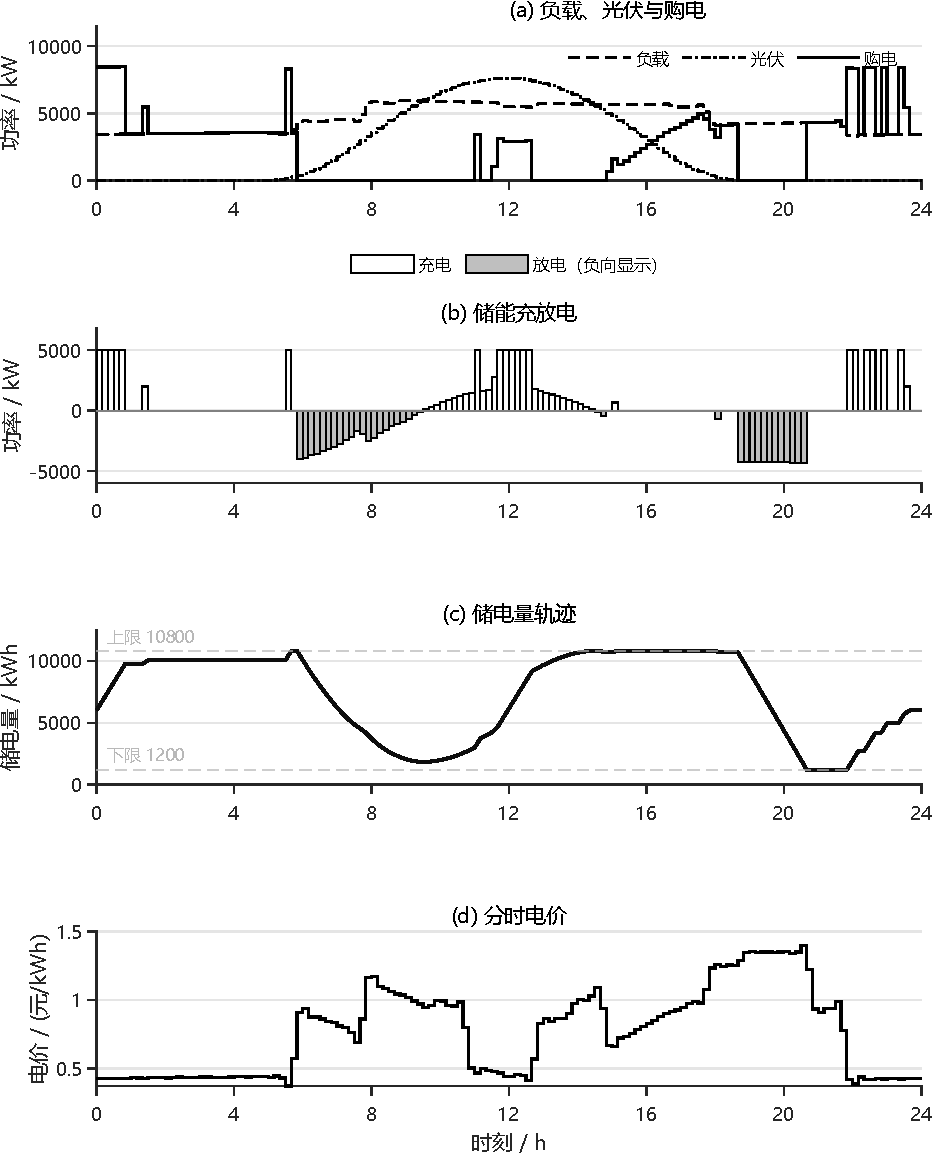
\includegraphics[width=.93\textwidth,height=.65\textheight,keepaspectratio]{figures/q1_dispatch.pdf}
\caption{问题一的购电、充放电及储电量轨迹。放电在图中负向显示，其模型变量仍为非负电量。}\label{fig:q1}
\end{figure}
